% Appendix: supplementary figures moved out of the main text in the JFM narrative
% cull (Session 29.2). These are diagnostic / qualitative panels referenced from
% the Results: the qualitative rollout traces, the per-axis error map, and the
% decode-ceiling vorticity panels. They support the main claims but are not
% themselves narrative steps, so they live here to keep the main figure set tight.

The figures below are referenced from the Results and collected here to keep the
main-text figure sequence focused on the narrative steps. They are diagnostic and
qualitative: the predictor rollout traces (figure~\ref{fig:traces}), the per-axis
breakdown of the paired wake advantage (figure~\ref{fig:error_maps}), and the
decode-ceiling vorticity panels (figure~\ref{fig:recon}).

\begin{figure}
  \centering
  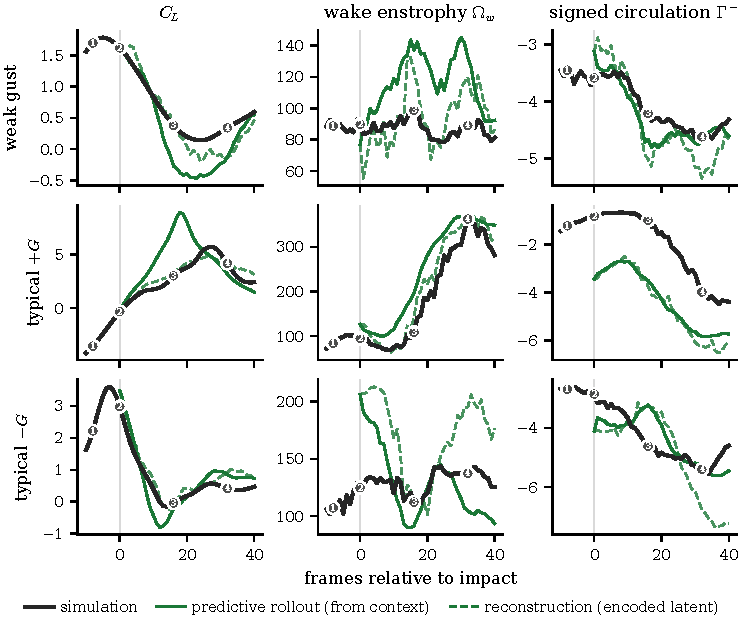
\includegraphics[width=\linewidth]{sections/figures/results/figA_traces_v2p1.pdf}
  \caption{The predictive rollout tracks the encounter, shown qualitatively.
  Predicted observables through representative held-out encounters (rows), for the
  lift coefficient, the wake enstrophy, and the negative circulation (columns). The
  simulation is the bold reference; the rollout of the predictor, started from the
  pre-impact context, is the coloured line, and the dashed line is the
  reconstruction from the encoded latent. The rollout tracks the
  wake observables through the leading-edge-vortex peak and into recovery before
  drifting gently at long times. We report this as qualitative tracking, not as a
  closure $R^2$. Numbered glyphs mark the four encounter stages used throughout:
  baseline, impact, peak load, and recovery.}
  \label{fig:traces}
\end{figure}

\begin{figure}
  \centering
  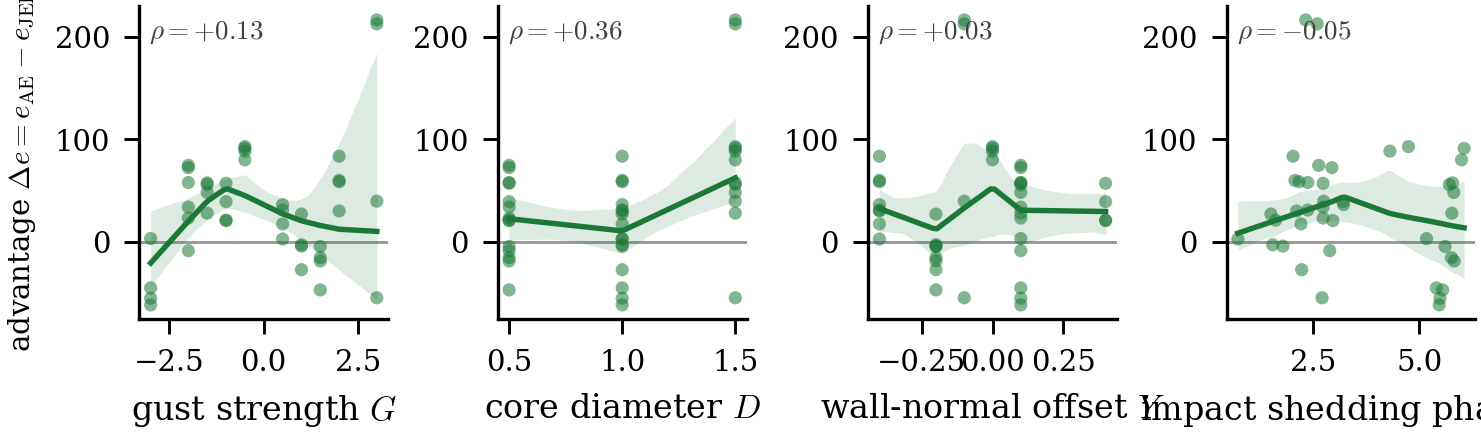
\includegraphics[width=\linewidth]{sections/figures/results/fig_error_maps_v2p1.png}
  \caption{Per-encounter paired improvement
  $\Delta e = e_{\text{AE}} - e_{\text{JEPA}}$ in held-out wake-enstrophy error
  against the gust strength $G$, core diameter $D$, wall-normal offset $Y$, and
  the baseline shedding phase at impact $\phi$ (test\_b, $n = 42$); positive
  $\Delta e$ means the predictive latent carries the smaller error. Each panel
  shows the per-encounter values, a locally weighted (LOWESS) trend, and a
  bootstrap band over encounters. The predictive advantage grows with $D$
  (significant) but shows no significant $G$ or $Y$ trend; the shedding-phase axis
  falls into two clusters because impact is fixed near a single convective instant.}
  \label{fig:error_maps}
\end{figure}

\begin{figure}
  \centering
  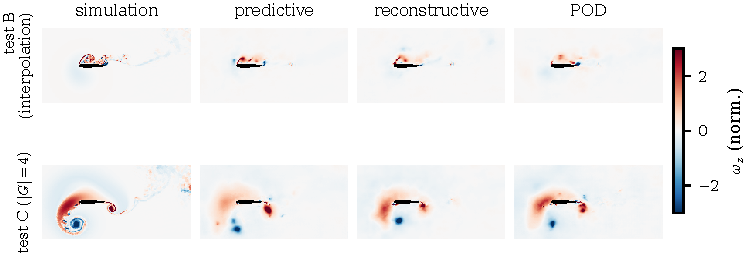
\includegraphics[width=\linewidth]{sections/figures/results/figD_reconstructions_v2p1.pdf}
  \caption{Decoded vorticity at the impact frame on held-out encounters (rows: an
  interpolation test\_b encounter and a $|G| = 4$ test\_c encounter) for the
  simulation and the predictive, reconstructive, and POD decodes (columns). The
  predictive decoder is blurry by design but localises the impingement; the
  reconstructive autoencoder collapses toward a near-uniform field on the held-out
  interpolation condition, while the linear basis is amplitude-accurate. All
  families degrade in the $|G| = 4$ regime, reported as the observability boundary
  of \S\ref{sec:flow_physics} rather than as a generalisation claim. Field-space
  similarity is read only as a labelled decode ceiling (\S\ref{sec:res_physical}).}
  \label{fig:recon}
\end{figure}

\begin{figure}
  \centering
  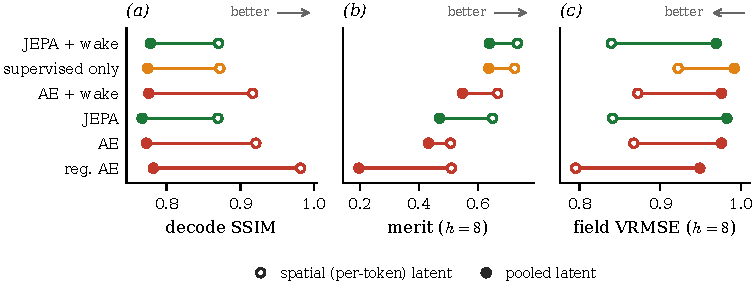
\includegraphics[width=\linewidth]{sections/figures/results/fig_pooling_cost_v3.pdf}
  \caption{The decodability-versus-estimability trade of
  \S\ref{sec:disc_decode}, quantified. Each panel connects the spatially
  resolved latent (open marker) to its pooled coefficient state (filled marker),
  per family, for the decode similarity, the matched-predictor merit, and the
  field forecast error. Pooling costs field fidelity in every family; the
  coefficient state is the price of a state a wall-pressure filter can track.}
  \label{fig:pooling_cost}
\end{figure}
